\chapter{Design und Implementierung}
\label{cha:DesignUndImplementierung}

Im letzten Kapitel wurde der Ablauf eines Testprojekts aufgezeigt und eine Einführung in das Thema \enword{Keyword-Driven-Testing} gegeben. In diesem Kapitel wird das Rayden-System detailiert erklärt. Am Anfang diese Kapitel werden die Designziele der Sprache-Rayden erklärt. Die Sprache-Rayden ist eine domänenspezifische Sprache und hat einige Eigenheiten und Überraschungen. In den weiteren Abschnitten wird der Aufbau des Rayden-Systems erklärt und auf die technischen Details eingegangen. Am Ende diese Kapitel wird noch die Integration in die \enword{Java-Scripting-API} beschrieben. Das Rayden-System bietet die Möglichkeit, dass man einen Test in einer Java-Anwendung über das \enword{Java-Scripting-API} ausführen kann.

\section{Designziele von Rayden}

Das primäre Designziel von Rayden ist Offenheit. Rayden soll im gesamten Testprozess einsetztbar sein, aber darf die Personen nicht überfordern. Um dieses Ziel zu erreichen, setzten das Rayden-System auf mehreren Ebenen an.

\SuperPar
Die domänenspezifische Sprache von Rayden wird speziell für Personen im Testbereich entwickelt. Das wichtigste Ziel der Sprache ist Einfachheit. Die Sprache soll Personen ohne Programmierkenntnisse in die Lage versetzten, Tests in dieser Sprache zu lesen und zu bearbeiten. Die Sprache Rayden ist daher stark an der natürlichen Sprache angelehnt um den Einstieg zu erleichtern. Ein anderes Ziel bei dem Sprachdesign ist die Flexibilität der Sprache. Der Testprozess setzt sich aus einer Vielzahl an unterschiedlichen Aufgaben zusammen. Um möglichst alle Aufgaben mit der Sprache abdecken zu können, wird eine hohe Flexibilität benötigt. 

\SuperPar
Abgesehen von der Sprache gibt es noch weitere wichtige Ziele. Rayden wird plattformunabhängig entwickelt um viele Anwendungsszenarien abdecken zu können. Aus diesem Grund wird die Programmiersprache \enword{Java} für die Entwicklung des Rayden-Systems gewählt. Der Interpreter für Rayden selbst läuft auch wieder auf der \enword{Java-Virtual-Machine} laufen.

\SuperPar
Die Einbindung von externen Test-Treiber-Bibliotheken wird durch eine offene Schnittstelle ermöglicht. Dadurch können mit Rayden Tests für die unterschiedlichsten Anwendungsszenarien entwickelt werden. Rayden kann somit für das jeweilige Projekt und die beteiligten Personen angepasst werden. 

\section{Aufbau des Rayden-Systems}

In diesem Abschnitt wird der Aufbau des Rayden-Systems von zwei Blickwinkel beleuchtet. Zuerst wird der konzeptionelle Aufbau erklärt. Dabei wir darauf eingegangen, wie die einzelnen Konzept-Ebenen miteinander kommunizieren und welche Person für die jeweilige Ebene verantwortlich ist. Im zweiten Schritt wird die technische Architektur des Rayden-Systems erläutert. Dazu werden die Komponenten und ihre Beziehungen überblicksweise erklärt. Eine ausführliche Beschreibung findet man in den nächsten Abschnitten.

\subsection{Konzeptioneller Aufbau}

Wie schon in vorigen Abschnitten erwähnt, ist Rayden an das Konzept von \enword{Keyword-Driven-Testing} angelehnt. Deshalb ist es am Anfang interessant, wie der konzeptionelle Aufbau von \enword{Keyword-Driven-Testing} aussieht. 

\begin{figure}[h]
\centering
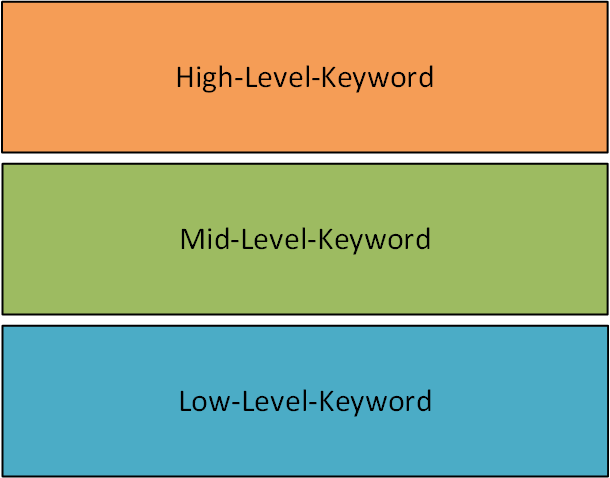
\includegraphics[width=0.7\textwidth]{KDT-Architektur.png}
\caption{Aufbau von \enword{Keyword-Driven-Testing}}
\label{fig:kdt-arch}
\end{figure}

\SuperPar
Ein \enword{Keyword-Driven-Test} besteht aus einer Sequenz von \enword{Keywords}. Diese \enword{Keywords} können wiederum aus einer Sequenz von \enword{Keywords} bestehen oder an einen Code gebunden sein. Die \enword{Keywords} werden in drei Kategorien, wie in Abbildung \ref{fig:kdt-arch} gezeigt wird, aufgeteilt. Die \enword{High-Level-Keywords} repräsentieren einen Testfall mit einer detaillierten Beschreibung. Diese Gruppe von \enword{Keyword} wird typischerweise von einer Person aus der Fachabteilung oder von einer Testmanagerin oder einem Testmanager erstellt. Dabei wird aber nur der Rumpf des \enword{Keywords} erstellt. Die Implementierung wird erst in der nächsten Phase hinzugefügt. Diese \enword{High-Level-Keywords} bilden die Grundlage für die Erstellung der Tests. In der weiteren Phase werden diese \enword{Keyword} von Testerinnen und Testern umgesetzt.

\SuperPar
Die \enword{High-Level-Keywords} bestehen typischerweise aus einer Sequenz von \enword{Mid-Level-Keywords}. Diese Sequenz wird in der zweiten Phase erstellt. Normalerweise finden sich \enword{Mid-Level-Keywords} in diese Sequenz, es können aber auch \enword{Low-Level-Keywords} verwendet werden. Die verwendeten \enword{Mid-Level-Keywords} bestehen wiederum aus einer Sequenz von \enword{Mid-Level-Keywords} und \enword{Low-Level-Keywords}. Technisch gesehen gibt es keine Unterschied zwischen \enword{High-Level-Keywords} und \enword{Mid-Level-Keywords}. Die Unterscheidung ist nur in der Art der Verwendung. \enword{High-Level-Keywords} beschreiben genau einen Anwendungsfall der getestet werden soll. Hier wird kein Wert auf Wiederverwendung gelegt im Gegenteil zu \enword{Mid-Level-Keywords}.

\SuperPar
In der letzten Phase werden \enword{Low-Level-Keywords} mit Code verbunden. Der Code kann prinzipiell in jeder Programmiersprache geschrieben sein. Die Wahl der Programmiersprache hängt von dem verwendeten \enword{Keyword-Driven-Framework} ab. In diesen \enword{Keyword-Driven-Frameworks} werden häufig Skript-Sprachen verwendet. Der Vorteil von Skript-Sprachen liegt darin, dass der Code für die Ausführung des Tests nicht kompiliert werden muss.

\begin{figure}[h]
\centering
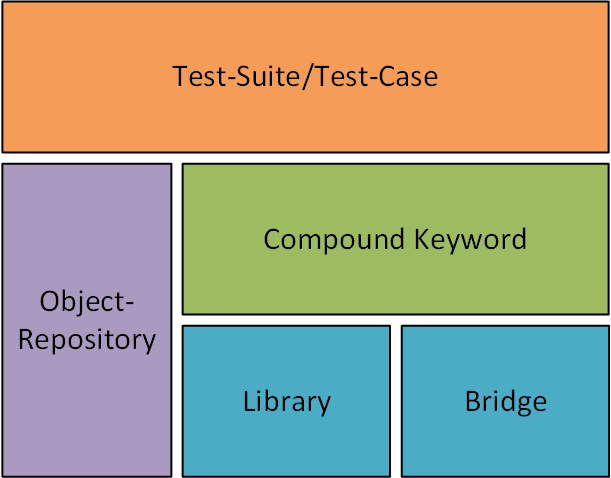
\includegraphics[width=0.7\textwidth]{Rayden-Architektur.png}
\caption{Aufbau von Rayden}
\label{fig:rayden-arch}
\end{figure}

\SuperPar
Im Gegensatz zu \enword{Keyword-Driven-Testing} unterteilt das Rayden-System die \enword{Keywords} in mehr Gruppen wie man in Abbildung \ref{fig:rayden-arch} sieht. Die zusätzlichen Gruppen bieten einen bessere Strukturierung und geben eine klare Richtung vor, wie ein Rayden-Test-Projekt aufgebaut werden soll.    

\SuperPar
Rayden führt eine klare Trennung bei \enword{Low-Level-Keywords} ein. Dies \enword{Keywords}, welche mit einem Code verbunden sind, werden in \enword{Library-Keywords} und \enword{Bridge-Keywords} unterteilt. \enword{Library-Keywords} stellen grundlegende Funktionen bereit, welche unabhängig von einem speziellen Anwendungsfall sind. Als Beispiel kann man sich eine \enword{For}- oder \enword{Print-Keyword} vorstellen. Im Gegensatz dazu sind \enword{Bridge-Keywords} speziell für eine Anwendungstechnologie angepasst wie z.B \enword{"`Open Browser"'} oder \enword{"`Navigate To"'} für Web-Anwendungen. 

\SuperPar
Auch bei den \enword{High-Level-Keywords} bietet Rayden eine größere Vielfalt. Grob werden diese in Test-Suiten und Testfälle unterteilt. Die Test-Suite dient als Gruppierungselement für Testfälle, um diese gemeinsam ausführen zu können. Bei der Definition von Testfällen können diese mit unterschiedliche Testtypen angelegt werden. Eine nähere Beschreibung findet man im Abschnitt \ref{cha:KeywordTypes}.

\SuperPar
Zum Abschluss ist noch auf das \enword{Object-Repository} hinzuweisen. Diese Komponente verwaltet Test-Objekte. Test-Objekte können für die Beschreibung von Benutzeroberflächen-Komponenten wie Schaltflächen oder Eingabefelder verwendet werden. Dafür wird für jedes Test-Objekt eine Bezeichner hinterlegt, mit welchem man die Komponente in der Benutzeroberfläche finden kann. Das ist im Fall einer Web-Anwendung ein \enword{XPath}- oder ein \enword{CSS}-Ausdruck. Das \enword{Object-Repository} sorgt somit für eine klare Trennung zwischen Test- und Benutzeroberflächen-Beschreibung. Diese Trennung erhöht die Wiederverwendbarkeit von \enword{Keywords} und reduziert den Wartungsaufwand bei Änderungen an der Benutzerschnittstelle.

\subsection{Technische Architektur}

Die technische Basis für das Rayden-System ist die Java-Plattform. Auf der Entwicklungsseite wird Java als Programmiersprache für das gesamte Rayden-System verwendet. Auf der Ausführungsseite läuft das Rayden-System auf der \enword{Java Virtual Machine}. Außerdem bietet Rayden die Möglichkeit, dass man einen Rayden-Test über das \enword{Java Scripting API}\cite{JavaScriptApi} ausführen kann. 

\begin{figure}[h]
\centering
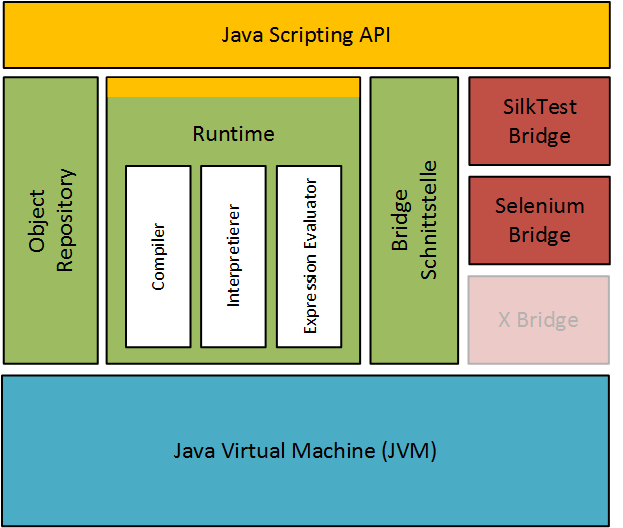
\includegraphics[width=0.9\textwidth]{Rayden-Tech-Architektur.png}
\caption{Rayden-Architektur}
\label{fig:rayden-tech-arch}
\end{figure}

\SuperPar
In Abbildung \ref{fig:rayden-tech-arch} sieht man alle Komponenten des Rayden-Kernsystems in Grün dargestellt. Diese Komponenten bilden die Grundlage, um einen Rayden-Test ausführen zu können. Als Basis dieser Komponenten sieht man in Blau die \enword{Java Virtual Machine}. Die externen \enword{Bridge}-Implementierungen werden in Rot dargestellt. Diese Komponenten stellen eine Verbindung zwischen dem Test-Treiber und der \enword{Rayden-Runtime} her und werden über die \enword{Bridge-Schnittstelle} hergestellt. Im oberem Abschnitt der Abbildung \ref{fig:rayden-tech-arch} sieht man das \enword{Java Scripting API}, über welches man Rayden-Tests ausführen kann.

\SuperPar
Im nächsten Absatz werden die einzelnen Komponenten der Rayden-Architektur beschrieben, um einen groben Überblick über die Funktionsweise von Rayden zu bekommen.\\

\begin{itemize}

\item \textbf{Runtime:}

Die \enword{Runtime} ist der Einstiegspunkt für die Ausführung in Rayden-Tests. Dazu beinhaltet diese Komponente die Implemntierung für die \enword{Java Scripting API}. Wird ein Test ausgeführt, werden zuerst alle Projektressourcen in der \enword{Runtime} geladen. Das Projektverzeichnis kann man über einen Kontextparameter setzen. Falls diese nicht gesetzt ist, wird der aktuelle Ordner verwendet. Für das Laden der Ressourcen wird die Compiler-Komponenten verwendet. Die \enword{Runtime} baut sich bei diesem Lesevorgang eine \enword{Lookup-Tabelle} für alle \enword{Keywords} auf. Die Tabelle wird für einen schnellen Zugriff im Interpreter benötigt. Der Rayden-Test wird mithilfe des Interpreters ausgeführt. Das Ergebnis des Tests wird als Resultat über die \enword{Java Scripting API} zurückgegeben.\\

\item \textbf{Compiler:}

Der Compiler für die Rayden-Sprache wurde mit dem Compiler-Werkzeug xText\cite{xtext} umgesetzt. Von dem generierten Compiler wird für die Ausführungseinheit nur der lexikalische und syntaktische Analysator verwendet. Der Eclipse-Editor wird für das Rayden-System nicht benötigt. Das Resultat der Compiler-Komponenten ist ein EMF-Modell des Tests. Die \enword{Runtime}-Komponenten verwaltet die Modelle und stellt diese dem Interpreter bei bedarf zur Verfügung.\\

\item \textbf{Interpreter:}

Der Interpreter ist die wichtigste Komponenten im Rayden-System. Der Interpreter ist dafür verantwortlich, dass die Rayden-Tests ausgeführt werden können. Zum Starten des Interpreter wird der Aufruf des \enword{Test-Keywords} übergeben. Diese \enword{Keyword} wird auf den leeren \enword{Stack} geladen. Der Test wird mithilfe einer \enword{Stack-Maschine}\cite{StackMachine} abgearbeitet. Bei jedem Aufruf von einem \enword{Keyword} wird die \enword{Keyword-Implementierung} auf den \enword{Stack} geladen. Zusätzlich wird für jeden neuen \enword{Keyword-Aufruf} ein neuer Gültigkeitsbereich(\enword{Scope}) angelegt. \\
\\
Der Gültigkeitsbereich ist für die Verwaltung der Parameter und Variablen zuständig. Eine Besonderheit in Rayden ist, dass Gültigkeitsbereiche vererbt werden. Eine detaillierte Beschreibung findet man im Abschnitt \ref{cha:KeywordScope}. Die Auswertung von Ausdrücken wird in einem separaten Teil des Interpreters vorgenommen. Für die Auswertung wird der aktuelle Gültigkeitsbereich und der Ausschnitt aus dem Modell an die Evaluierungskomponente übergeben. Das Ergebnis des Ausdrucks wird wieder auf den \enword{Stack} geladen. Ruft die \enword{Stack-Maschine} ein \enword{Scripted-Keyword}(Beschreibung in Abschnitt \ref{cha:KeywordMetaTypes}) auf, wird entweder der dazugehörige Code ausgeführt oder es wird der Aufruf an die \enword{Bridge-Schnittstelle} weitergeleitet.\\

\item \textbf{Bridge-Schnittstelle:}

Die \enword{Bridge-Schnittstelle} ist für die Anbindung von Test-Treibern verantwortlich. Um einen Test-Treiber verwenden zu können, muss eine \enword{Rayden-Bridge} implementiert werden. Die \enword{Bridge} mit der Schnittstelle bildet die Verbindung zwischen der \enword{Rayden-Runtime} und dem Test-Treiber.\\

\item \textbf{Object-Repository:}

Das \enword{Object-Repository} verwaltet Test-Objekte, welche von \enword{Keywords} verwendet werden können. Die Test-Objekte werden in einer Baumstruktur verwaltet. Als wichtigste Eigenschaft eines Test-Objekts ist der Bezeichner(\enword{Locator}). Mit dem Bezeichner kann Benutzerschnittstellen-Komponente identifiziert werden. Das Konzept ist an der Idee von \enword{Page-Object-Pattern}\cite{PageObject} angelehnt. \\

\end{itemize}


%%------------------------------------------------------------------------------------------------------

\section{Sprache von Rayden}

Als Inspiration und Basis für die Sprache dient das Konzept von \enword{Keyword-Driven-Testing}. Das Grundprinzip hinter \enword{Keyword-Driven-Testing} ist, dass ein Test aus mehreren \enword{Keywords} besteht. Diese \enword{Keywords} bestehen wiederum aus anderen \enword{Keywords} oder sind mit einem Code verbunden. Einen Test kann man auch als auch Baum darstellen, da keine Rekursionen in \enword{Keywords} erlaubt sind. 


Die Testsprache hat spezielle Eigenschaften. 
Keywords können als Sätze formuliert werden.
Die Sprache ist blockstrukturiert. Ist notwendig für die visuelle Darstellung.


TODO !!!

\section{Keywords}


\subsection{Metatypen von Keywords}
\label{cha:KeywordMetaTypes}

Scripted Keyword
Compound Keyword
Inline Keyword 
Scripted Compound Keyword

TODO !!!

\subsection{Ausprägungen von Keywords}
\label{cha:KeywordTypes}

TestSuite
TestCase
Unit Test
Integration Test
API Test
AU Test
Manual AU Test

\subsection{Sichtbarkeit}
\label{cha:KeywordScope}

Sichtbarkeit von Variablen und Keywords
TODO !!!

 Das Resultat davon ist, dass jeder Kind-Gültigkeitsbereich zugriff auf den Eltern-Gültigkeitsbereich hat. Der Vorteil davon ist, dass nicht alle Variablen übergeben werden müssen, da dies bei einem Test schon viele sein können. Es gibt auch die Möglichkeit, dass man explizit Parameter für ein \enword{Keyword} definiert. Das wird verwendet um sicher zu stellen, dass eine Variable zur Verfügung steht.

\section{Typsystem}

TODO !!!

\subsection{Parameter}

IN, OUT, INOUT

TODO !!!

\section{Verarbeiten von Keywords und Ausdrücke}

Keywords werden von einer Stackmaschine ausgeführt!

Ausdrücke werden nicht von der Stackmaschine ausgewertet sonderen haben eine eigene Ausführungseinheit. 
Diese Engine kann typsiert werden und verhält sich da durch bei Variables anders!

TODO !!!

\section{Library}

TODO !!!

\section{Bridge}

TODO !!!

\section{Object Repository}

%% UI Control Coverage 
%% Ableiten von neuen Tests

\section{Skript-Engine}

Die Java ScriptEngine Implementierung erkären

TODO !!!